\section{Oppsumering Møte 30.April}
\subsection{Plotting med \textsc{Python}}
For å lese filer med pyton er det best å bruke \texttt{numpy.loadtxt(file.dat)}.


\subsection{Truncation Ratio}
%
\begin{figure}[h!]
  \centering
   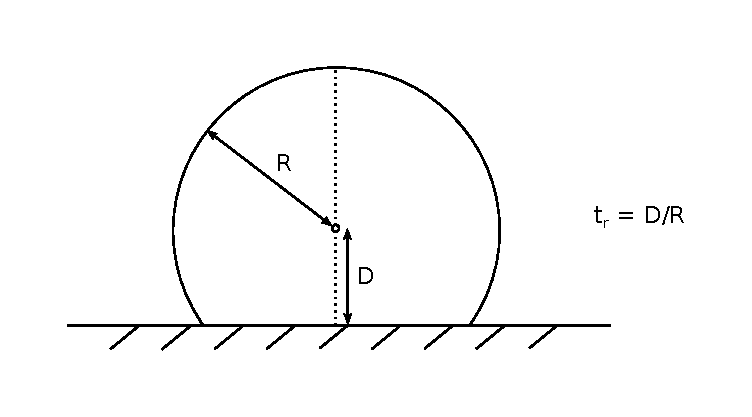
\includegraphics[width=0.5\textwidth]{truncationRatio.pdf}
   \caption{
   The geometrical meaning of the truncation ratio.
   }
   \label{fig:energyComparison}
\end{figure}
%


\subsection{Running Granfilm with -py option}
Skriv 
\begin{lstlisting}[style=FormattedNumber, language=bash]
./GranFilm
\end{lstlisting}
for å se hvilke parametere/flag du kan kjøre prøgrammet med.
\\
\\
Ved å bruk flagget \texttt{-py}, e.g.:
\begin{lstlisting}[style=FormattedNumber, language=bash]
./GranFilm  -py  -p parameters.sif -o output.dat
\end{lstlisting}
får man ekstra ''output''-filer, blant annet \texttt{output.dat\_RefTrans}, se Tabell \ref{tab1}.
%
\begin{table}[htbp]
   \caption{Eksempel på ekstra output data output.dat\_Ref. Fresnel dataen er 
   hva refleksjons koeffisienten er hvis substratet hadde vært bart (flatt, uten dråper)}
\centering
\begin{tabular}{ c c c c }
\hline
 \multicolumn{2}{c}{r\_p}         &  \multicolumn{2}{c}{r\_p fresnel} \\
\hline
$\Re$\{r\_p\}  &  $\Im$\{r\_p\} & $\Re$\{r\_p fresnel\}   & $\Im$\{r\_p fresnel\}  \\
$\downarrow$ & $\downarrow$ &  $\downarrow$         &    $\downarrow$ \\
            &              &              &              \\
\hline
\end{tabular}
\label{tab1}
\end{table}
%
